% `advanced_example.tex', an advanced example employing the AIAA class
% plus other third-party LaTeX packages.
%
% For a bare-bones usage, see `template.tex'.
%
% Typical processing for PostScript (PS) output:
%
%  latex advanced_example
%  bibtex advanced_example  (bibliography)
%  makeindex -s nomencl.ist -o advanced_example.gls advanced_example.glo
%                            (nomenclature)
%  latex advanced_example   (repeat as needed to resolve references)
%
%  xdvi advanced_example    (onscreen draft display)
%  dvips advanced_example   (postscript)
%  gv advanced_example.ps   (onscreen display)
%  lpr advanced_example.ps  (hardcopy)
%
% With the above, only Encapsulated PostScript (EPS) images can be used.
%
% Typical processing for Portable Document Format (PDF) output:
%
%  pdflatex advanced_example
%  bibtex advanced_example    (bibliography)
%  makeindex -s nomencl.ist -o advanced_example.gls advanced_example.glo
%                              (nomenclature)
%  pdflatex advanced_example  (repeat as needed to resolve references)
%
%  acroread advanced_example.pdf  (onscreen display)
%
% If you have EPS figures, you will need to use the epstopdf script
% to convert them to PDF because PDF is a limmited subset of EPS.
% pdflatex accepts a variety of other image formats such as JPG, TIFF,
% PNG, and so forth -- check the documentation for your version.
%
% If you do *not* specify suffixes when using the graphicx package's
% \includegraphics command, latex and pdflatex will automatically select
% the appropriate figure format from those available.  This allows you
% to produce PS and PDF output from the same LaTeX source file.
%
% To generate a large format (e.g., 11"x17") PostScript copy for editing
% purposes, use
%
%  dvips -x 1467 -O -0.65in,0.85in -t tabloid advanced_example
%
% For further details and support, read the Users Manual, aiaa.pdf.

\documentclass[]{aiaa-tc}% insert '[draft]' option to show overfull boxes

 \usepackage{varioref}%  smart page, figure, table, and equation referencing
 \usepackage{wrapfig}%   wrap figures/tables in text (i.e., Di Vinci style)
 \usepackage{threeparttable}% tables with footnotes
 \usepackage{dcolumn}%   decimal-aligned tabular math columns
  \newcolumntype{d}{D{.}{.}{-1}}
 \usepackage{nomencl}%   nomenclature generation via makeindex
  \makeglossary
 \usepackage{subfigure}% subcaptions for subfigures
 \usepackage{subfigmat}% matrices of similar subfigures, aka small mulitples
 \usepackage{fancyvrb}%  extended verbatim environments
  \fvset{fontsize=\footnotesize,xleftmargin=2em}
 \usepackage{lettrine}%  dropped capital letter at beginning of paragraph
 \usepackage[dvips]{dropping}% alternative dropped capital package
 \usepackage[colorlinks]{hyperref}%  hyperlinks [must be loaded after dropping]

 \title{Advanced Example of AIAA Technical Conference Paper}

 \author{
  First A. Author\thanks{Job Title, Department, Address, and AIAA Member Grade.}
  \ and Second B. Author\thanksibid{1}\\
  {\normalsize\itshape
   Business or Academic Affiliation, City, Province, Zipcode, Country}\\
  \and
  Third C. Author\thanks{Job Title, Department, Address,
                         and AIAA Member Grade.}\\
  {\normalsize\itshape
  Business or Academic Affiliation, City, Province, Zipcode, Country}
 }

 % Data used by 'handcarry' option
 \AIAApapernumber{YEAR-NUMBER}
 \AIAAconference{Conference Name, Date, and Location}
 \AIAAcopyright{\AIAAcopyrightD{YEAR}}

 % Define commands to assure consistent treatment throughout document
 \newcommand{\eqnref}[1]{(\ref{#1})}
 \newcommand{\class}[1]{\texttt{#1}}
 \newcommand{\package}[1]{\texttt{#1}}
 \newcommand{\file}[1]{\texttt{#1}}
 \newcommand{\BibTeX}{\textsc{Bib}\TeX}

\begin{document}

\maketitle

\begin{abstract}
This is the advanced example employing \LaTeX\ to produce an AIAA
technical conference paper.
Please read the Known Problems in the Users Manual before attempting
to use this example as a template.
Fundamental topics are covered in the bare-bones template.
For detailed AIAA layout and style guidelines, please refer to the AIAA
\LaTeX\ Package Users Manual, \file{aiaa.pdf}.
\end{abstract}

\printglossary% creates nomenclature section produced by MakeIndex

\section{Introduction}

\lettrine[nindent=0pt]{T}{his} is an example of a dropped capital letter
at the beginning of a paragraph using the \package{lettrine} package.
This package is usually included with the more comprehensive \TeX\
distributions, but those with more trim installations may need to
retrieve this package from the Comprehensive \TeX\ Archive Network
(CTAN), which is located at \href{http://www.ctan.org}{www.ctan.org}.
This package does not gracefully handle the AIAA class' \verb|submit|
option.

\dropping{2}{A}{\textsc{nd}} this is an example of a dropped capital
letter at the beginning of a paragraph using the \package{dropping}
package.
This package is a bit less refined than the \package{lettrine} package,
but some authors may already have it around if they used the old
(unofficial) \LaTeX\ AIAA distribution.
This package accommodates the AIAA class' \verb|submit| option.

\begin{wrapfigure}{R}{0.3\linewidth}
 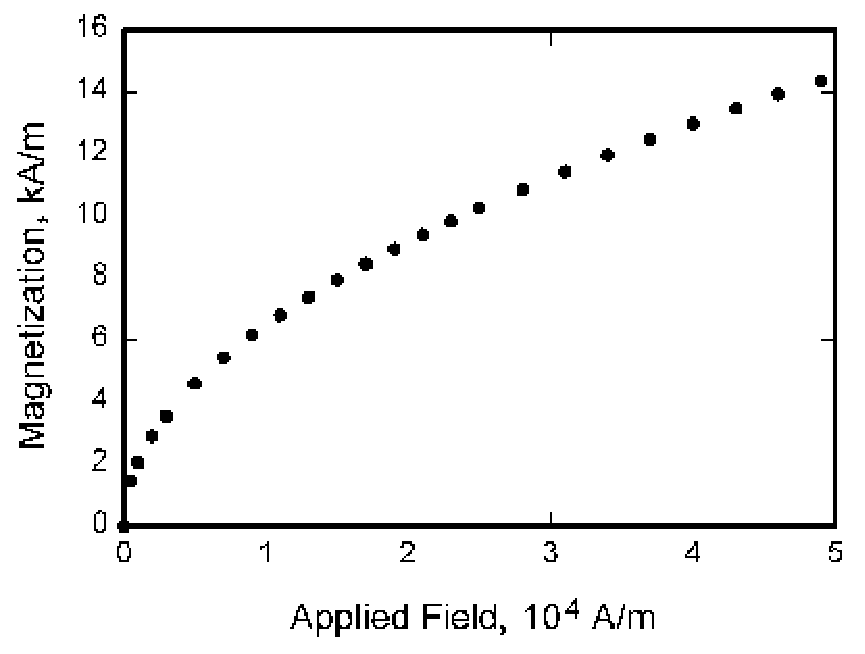
\includegraphics{figure_magnet}
 \caption{Magnetization as a function of applied field.}
 \label{f:magnetic_field}
\end{wrapfigure}

In an effort to more tightly integrate text and image, the
\package{wrapfig} package is employed.
This package works by modifying paragraph shape to accommodate a figure
(or a table or other items).
Typically one inserts its \verb|wrapfigure| or \verb|wraptable|
environment just before the paragraph in which it is to be placed.
Also specified is the width of the item to be inserted and the
placement, for example, left or right side.
(This package does not provide for center placement.)
The rest of this paragraph is filler so that the \verb|wrapfigure|
example will be placed in this paragraph.
Documentation of the \package{wrapfigure} package is available at the
end of the style file itself (check the package loading lines shown
during \LaTeX\ processing to find its location).

Code listings and other such artifacts can be typeset in a large variety
of styles by using the \package{fancyvrb} package.
\begin{Verbatim}[numbers=left]
 def testCircularAdvection
  position.each_index do |i|
   @position = position[i]
   assert_equal speed[i], waveSpeed
  end
 end
\end{Verbatim}

Tables with footnotes, such as table~\vref{t:threepart},
can be coded using the \package{threeparttable} package.
Note: This table was purposely placed on another page through the use of
the \verb|[p]| placement specifier to demonstrate the automated page
reference mechanism provided by the \package{varioref} package.
Of course, one would normally have the table integrated into the text
that describes it.
\begin{table}[p]
 \begin{center}
  \begin{threeparttable}
   \caption{This is an example of a \package{threeparttable} which uses the
     \package{dcolumn} package to allow for columns to be aligned on decimal
     points.}
   \label{t:threepart}
   \begin{tabular}{lcdd}
    First head\tnote{*}  &
    Second head &
    \multicolumn{1}{c}{Third head} &
    \multicolumn{1}{c}{$V_M(r)$} \\\hline
    center & doctor &  0.2  & 10.55 \\  
    tab    & dentist &  0.15 & 33.12 \\ 
    worse  & man\tnote{\ensuremath{\dagger}} & 10.58 & 45.10 \\ 
    better & home & 43.9  & 12.34 \\
   \end{tabular}
   \begin{tablenotes}
    \item[*] This is a table footnote, which to span multiple lines, has
      been greatly extended in length contrary to reason.
    \item[\ensuremath{\dagger}] A much shorter table footnote.
   \end{tablenotes}
  \end{threeparttable}
 \end{center}
\end{table}

Equation~\eqnref{e:displace} is serving as a demonstration of the
\package{nomenclature} package.
\begin{equation}
  \label{e:displace}
  \mathbf{J}_i\cdot\Delta\underline{x}_{i+1}=-\underline{f}_i
\end{equation}%
\nomenclature{$J$}{Jacobian Matrix}%
\nomenclature[b$i$]{$i$}{Variable number}%
\nomenclature[g$\Delta$]{$\Delta x$}{Variable displacement vector}%
\nomenclature{$f$}{Residual value vector}%
\nomenclature{$x$}{Variable value vector}%
The same can be said for Eq.~\eqnref{e:newton} that uses $\alpha$ to add
another Greek letter to the mix.
\begin{equation}
  \label{e:newton}
  F=m\alpha
\end{equation}%
\nomenclature{$F$}{Force, N}%
\nomenclature{$m$}{Mass, kg}%
\nomenclature[g$\alpha$]{$\alpha$}{Acceleration, m/s\textsuperscript{2}}%
The \package{nomencl} package is fed entries with the
\verb|\nomenclature| command.
These entries are then collected and sorted using \verb|makeindex|.
The optional sorting argument to the \verb|\nomenclature| command uses
a key of `b' for subscripts, `g' for Greek symbols, `c' for conventions,
and `t' for superscripts.

When many figures share a similar style and beg to be compared to one
another, the \package{subfigmat} and \package{subfigure} packages can be
used to create a matrix of subfigures as shown by
figure~\vref{f:small_multiple}.
\begin{figure}
 \begin{subfigmatrix}{4}% number of columns
  \subfigure[2 AM.]{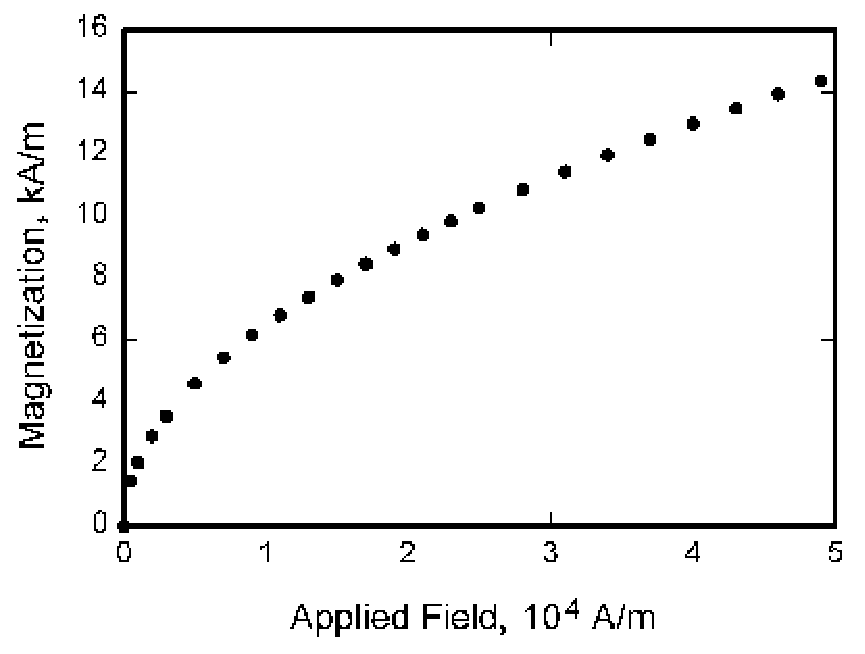
\includegraphics{figure_magnet}}
  \subfigure[3 AM.]{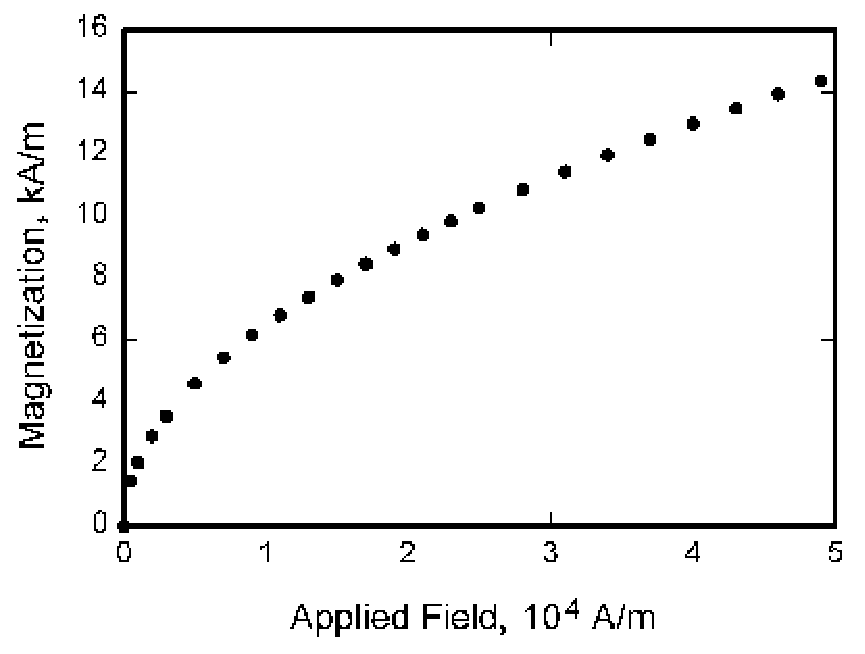
\includegraphics{figure_magnet}}
  \subfigure[4 AM.]{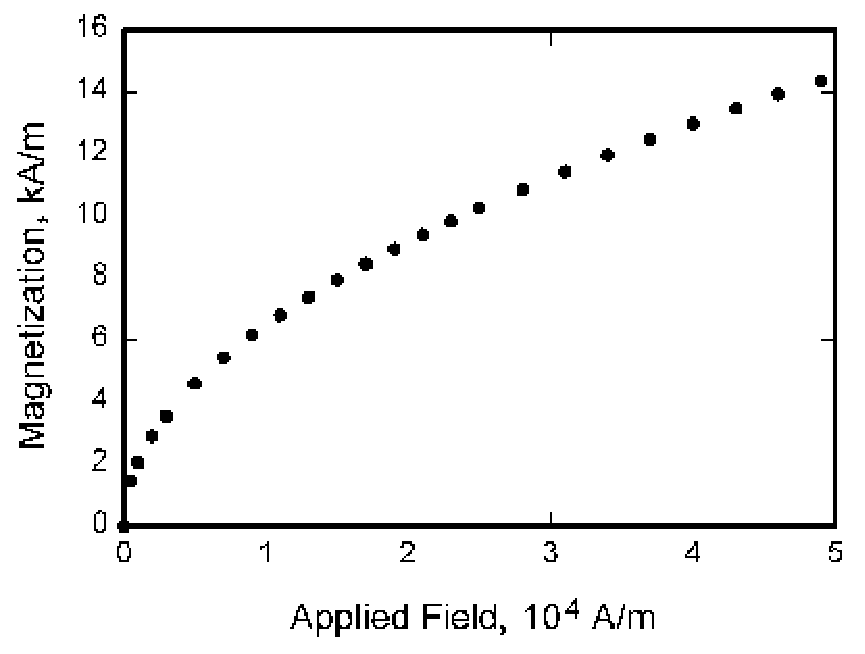
\includegraphics{figure_magnet}}
  \subfigure[5 AM.]{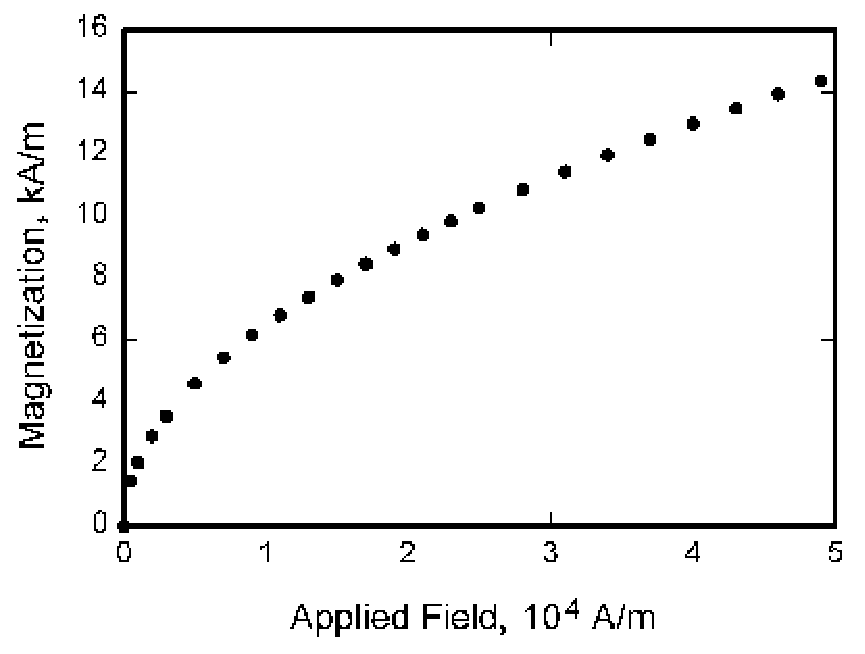
\includegraphics{figure_magnet}}
  \subfigure[6 AM.]{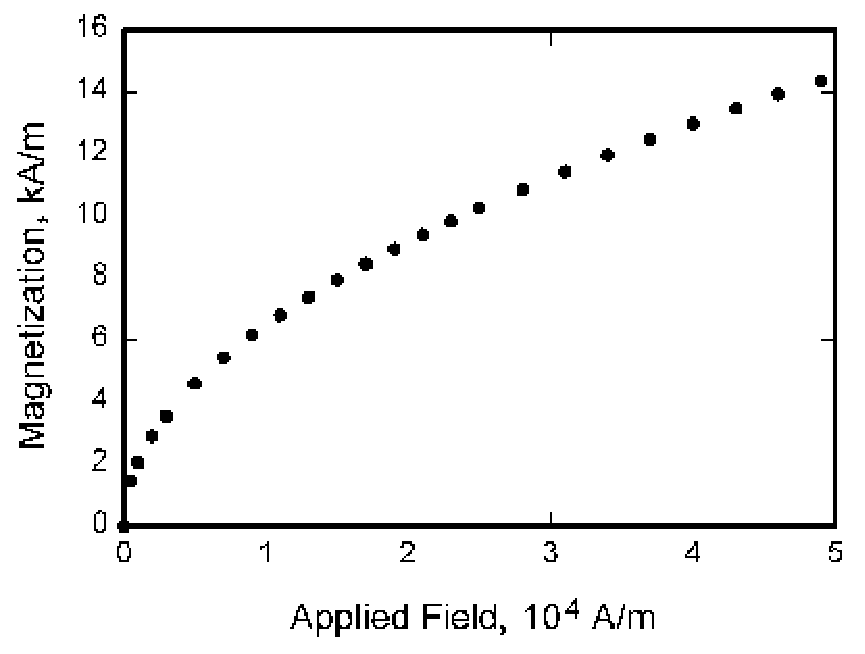
\includegraphics{figure_magnet}}
  \subfigure[7 AM.]{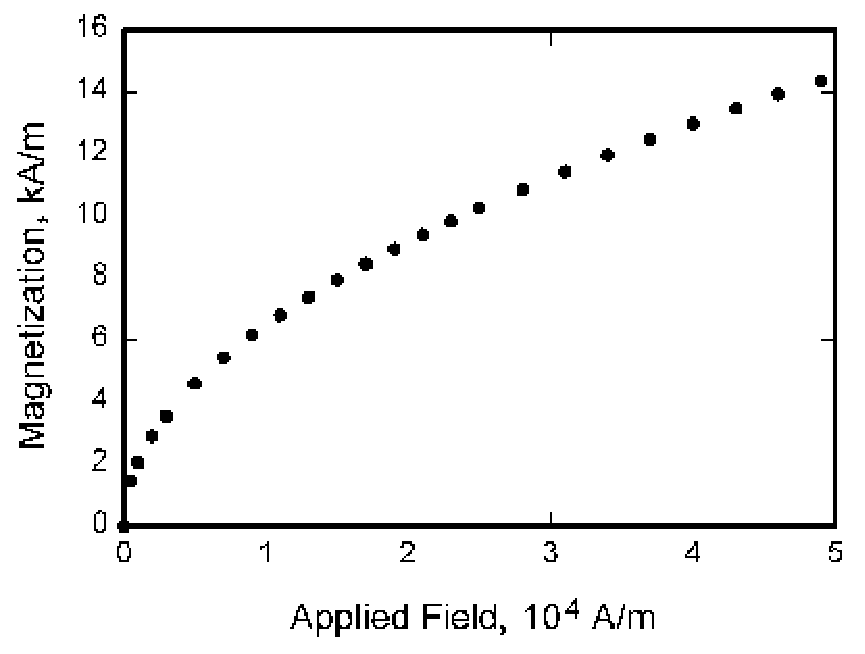
\includegraphics{figure_magnet}}
  \subfigure[8 AM.]{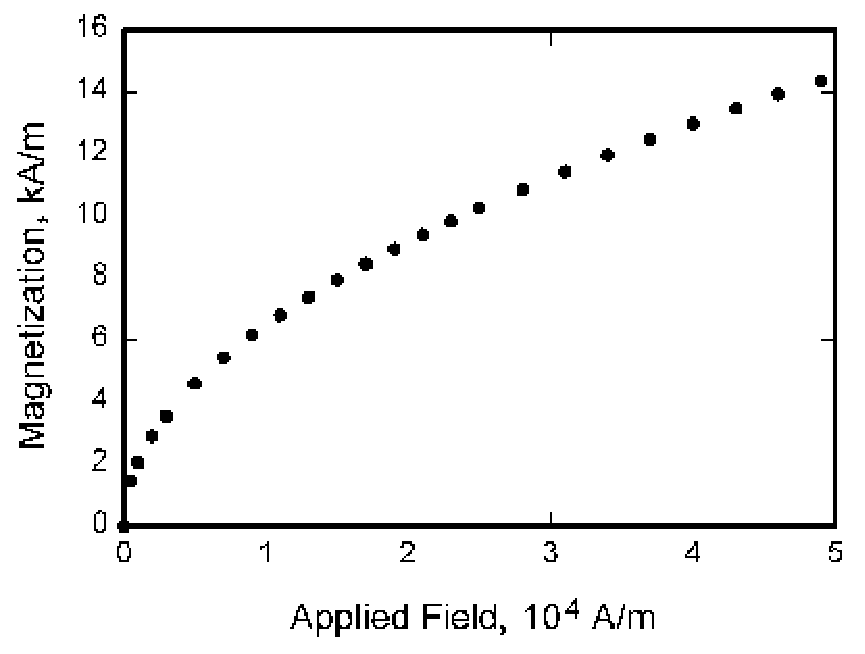
\includegraphics{figure_magnet}}
  \subfigure[9 AM.]{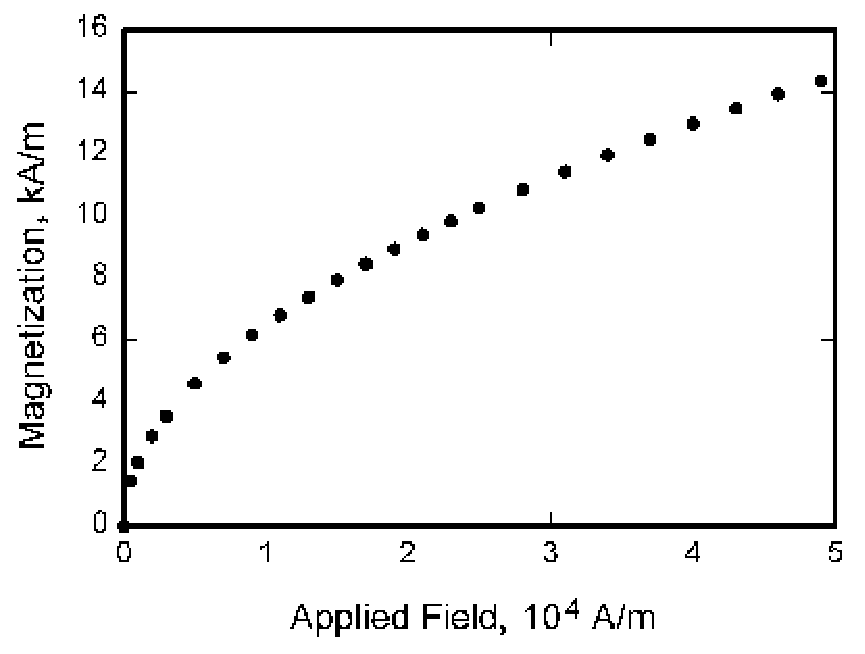
\includegraphics{figure_magnet}}
 \end{subfigmatrix}
 \caption{A time series shown of magnetic field that does not change
          because we are using the same figure each time.}
 \label{f:small_multiple}
\end{figure}
These are called ``small multiples'' by Tufte.\cite{tufte:83bk}

\section{Conclusion}

This had been a brief example of some of the more advanced options
available for \LaTeX.
Please see the documentation for each package for extended discussion or
usage.

% produces the bibliography section when processed by BibTeX
\bibliography{bibtex_database}
\bibliographystyle{aiaa}

\end{document}

% - Release $Name:  $ -

% Copyright - Carlos Montalvo 2015
% You may freely distribute this file but please keep my name in here
% as the original owner
